% hello.tex - Our first LaTeX example!
\documentclass[11pt]{article}
\usepackage[lmargin=0.5in, rmargin=0.5in,tmargin=1.0in,bmargin=1.0in]{geometry}
\usepackage{graphicx}
\usepackage{times}
\title{Physics Behind the Simulation: A CS296 Report by Group 31}
\author{Sai Charan\\
  120050060\\
  \texttt{saicharan@iitb.ac.in}\and
  Vinay Chandra\\
  120050063\\
  \texttt{vinaychandra@iitb.ac.in}\and
  Nikhil Sri Ram\\
  120050070\\
  \texttt{nikhil007@iitb.ac.in}\\
}
\date{\today}

\begin{document}

\maketitle
\section{Introduction}
This report is to explain the physics of the extra three objects that are newly added to the existing simulation on Box2D. The three additions to the previous simulation are  two rotating rods \bf X \rm, \bf Y \rm, a ball \bf B \rm and a set of dominos \bf D \rm, of which \bf B \rm and \bf D \rm are kept on a new horizontal base.

\section{Physics behind the Simulation}
The open box filled with the small spheres comes down due to the weight of those balls, and on its way down collides with both the rotating rods. These rods are placed such that one disturbs the dominos and the other one disturbs the ball.

\subsection{Rotating Rods}
This part consists of two rectangular blocks \bf X \rm, \bf Y \rm elongated along lengthwise pinned at the centre of the block thereby reducing the number of degrees of freedom to one (one along rotation). The rods are inelastic(ie.,coefficient of restitution = 0) 

Once the open box is filled with enough balls to overcome the counter weight, the open box accelarates downwards with acceleration \bf `a' \rm  given by :-\begin{equation} a = {(m_1-m_2)\over (m_1+m_2)} g \end{equation}
Assume that velocity of the box once it reaches the rotating rod be \bf`v'\rm. The heights of the rods are chosen such that the box collides with both of the rods simultaneously. After collision let the velocity of open box \bf O \rm be v1 and that of the rods be vx, vy at the point of contact[v1=vx=vy because the objects are inelastic \cite{rsk}]. Let masses of the rods be mx, my.

\centerline{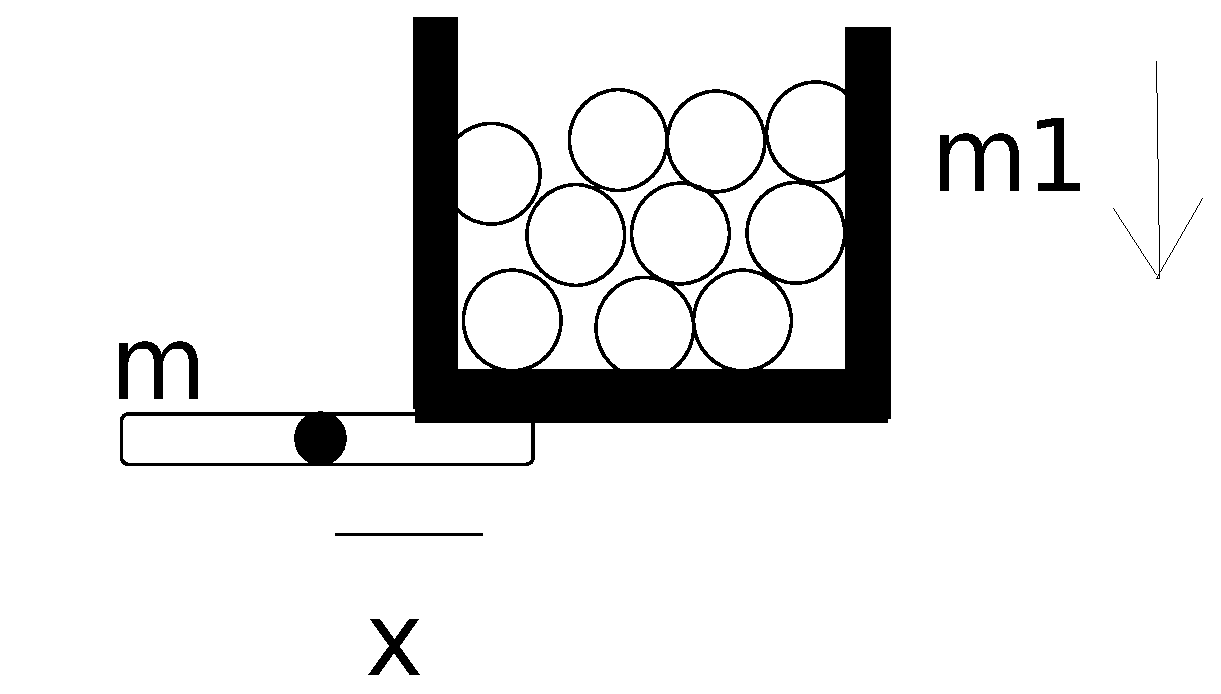
\includegraphics[scale=0.1]{1}}

The equations governing the collision are\begin{equation}m_1v - m_1*v_1 = J_1 + J_2\end{equation}\begin{equation}J_1*x = m_xl_xv_1/12 \end{equation}\begin{equation}J_2*x = m_y.l_y.v_1/12 \end{equation}
Here in the above equations J1,J2 are impulses acted upon rotating rod \bf X \rm, rotating rod \bf Y \rm and open box \bf O \rm respectively.for more on collisions refer \cite{hcv}
\\
\\
\centerline{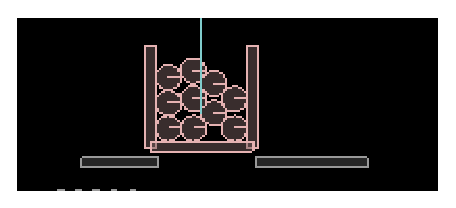
\includegraphics[scale=0.9]{11}}



\subsection{Dominos}
Interesting part of physics can be found in the simulation of dominos. The whole physics can be divided into two parts. One, the collision that takes place between the rotating rod \bf X \rm and the first domino. This collision induces angular momentum as well as linear momentum for the first domino, thereby the domino rotates as well as translates.As the domino rotates, the rotating motion accelerates by the influence of gravity, thereby picking up more angular momentum[about the base of the domino] than which it started with, before it collides with the next. It is because of this mechanism that the process of falling dominos speeds up.\\
\centerline{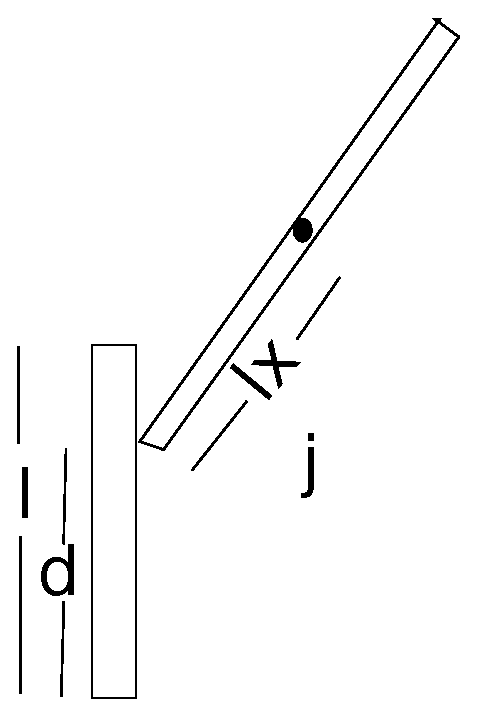
\includegraphics[scale=0.2]{2}}\\

The equations governing this part are
\begin{equation}J*d=m_dl^2w/3\end{equation}
J is the impulse imparted to the domino, l is the length of the domino, m*l*l/3 is the moment of inertia about the bottom of the domino(refer parallel axis theorem in \cite {dcp})
\begin{equation}w_1*l_x*cos\theta=w*d\end{equation}
w1 is the final angular velocity of the rotating rod \bf X \rm, lx is the half-length of rod \bf X \rm, theta is the angle at which rod struck the domino, d is the distance of the point of contact from the base of the domino.
\begin{equation}J*l_x*cos\theta=I*(v_1/l_x-w_1)\end{equation}
where the symbols carry the same meaning as from above
\\
\\
\centerline{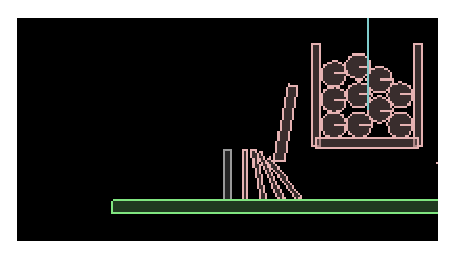
\includegraphics[scale=0.9]{12}}
For more on angular momentum refer \cite{hcv}




\subsection{The Ball}
The simplest part of the paper is this section. The rotating rod \bf Y \rm rotates and collides with the ball \bf B \rm, thereby mobilising the ball and during this collision the rotating rod \bf Y \rm simultaneously slows down.\\
\\
\centerline{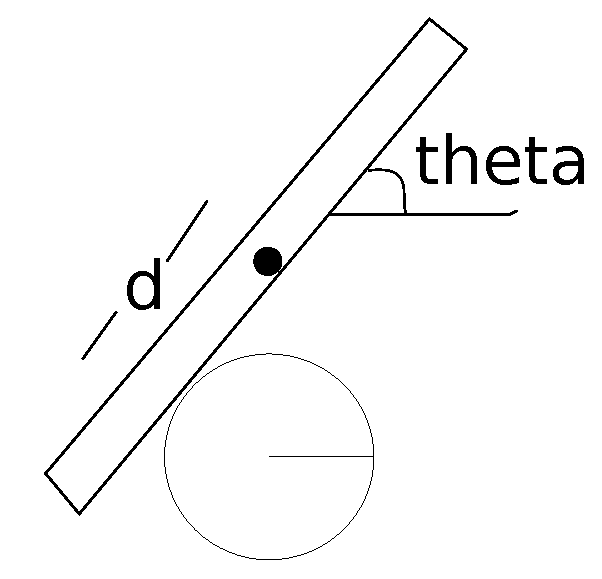
\includegraphics[scale=0.2]{3}}\\
The equations for this part are similar to that of the above part except for there is no domino action in this case.\\
\begin{equation}Jcos\theta*d=m_yl_y^2/12(w - w_2) \end{equation}
J is the impulse imparted to the ball(as well as on the rod, by Newton's 3rd law), ly is the half-length of the rod, my*l*l/12 is the moment of inertia about the center of the rod
\begin{equation}w_2*d*cos\theta=v_b\end{equation}
w2 is the final angular velocity of the rotating rod \bf Y \rm, ly is the half-length of rod \bf Y \rm, theta is the angle at which rod struck the domino, d is the distance of the point of contact from the center of the rod, vb is the final velocity of the ball
\begin{equation}J=m_b*v_b\end{equation}
where the symbols carry the same meaning as from above
\\
\\
\centerline{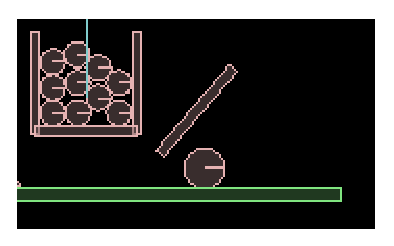
\includegraphics[scale=0.9]{13}}
\bibliographystyle{plain}
\bibliography{cs296_report_31}
\end{document}
